\documentclass[12pt]{article}
\usepackage[a4paper, total={7.5in, 11in}]{geometry}
%\usepackage{array}
\usepackage{graphicx, subfig, wrapfig, fancyhdr, lastpage, multicol ,color, mhchem}
\newcommand\headerMe[2]{\noindent{}#1\hfill#2}
\usepackage[mathscr]{euscript}
\usepackage{tabularray}

\setlength{\columnseprule}{1pt}
\def\columnseprulecolor{\color{blue}}


\pagestyle{fancy}
\fancyhf{}

\cfoot{\vspace{-10cm} \em{Page \thepage \hspace{1pt} / \pageref{LastPage}}}
\begin{document}

\headerMe{Royaume du Maroc}{année scolaire \emph{2024-2025}}\\
\headerMe{Ministère de l'Éducation nationale, }{  Professeur :\emph{Zakaria Haouzan}}\\
\headerMe{du Préscolaire et des Sports}{Établissement : \emph{Lycée SKHOR qualifiant}}\\

\begin{center}
Devoir Surveillé  N°1 \\
    2ème année baccalauréat Sciences Mathématiques\\
Durée 2h00
\\
    \vspace{.2cm}
\hrulefill
\Large{Chimie 7pts/42min}
\hrulefill\\

    \emph{Les deux parties sont indépendantes}
\end{center}
%end Headerss------------------------
%__________________Chimie ______________________-
%%%%%%%+_+_+_+_+_+_+_+_+_Partie1

 \section*{Partie 1 :Contrôle et suivi temporels d’un mélange réactionnel
par titrage d’oxydoréduction  \dotfill(7pts) }


\begin{wrapfigure}[13]{r}{0.42\textwidth}
	\vspace{-1cm}
\begin{center}
  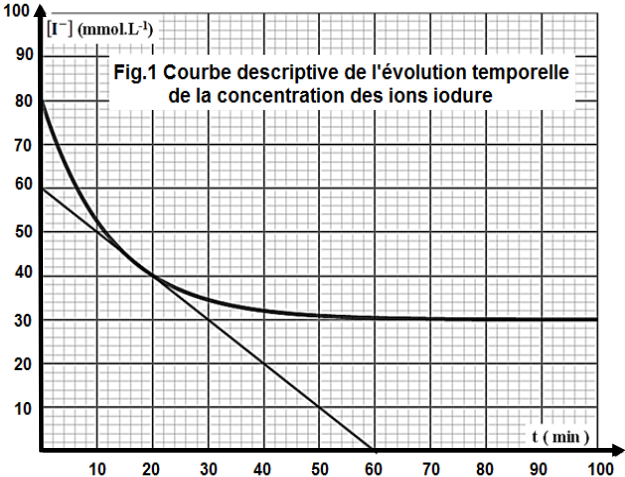
\includegraphics[width=0.42\textwidth]{./img/chimie_00.png}
\end{center}
\end{wrapfigure}



A la date $t = 0$, et à une température constante de $25^{\circ}C$ , on considère un premier système chimique préparé
en mélangeant un volume $V_1 = 50 mL$ d’une solution aqueuse de peroxodisulfate d’ammonium ($2NH^+_{4(aq)} + {{S_2O_8}^{2-}}_{(aq)}$
de concentration molaire $C_1 = 5.10^{-2} mol/L$
, un volume $V_2 = V_1$ d’une solution aqueuse d’iodure de potassium $(K^+_{(aq)} + I^-_{(aq)})$ de concentration molaire
  $C_2 = 3,2.C1$ et quelques gouttes d’une solution d’empois d’amidon fraîchement
préparé .On rappelle que l’empois d’amidon colore en bleu nuit une solution contenant du diiode $I_2$ même en faible
quantité. A une date t, on prélève, du mélange, un volume $V = 10 mL$ qu’on lui ajoute de l’eau glacée et on dose la
quantité de $I_2$ formée par une solution de thiosulfate de sodium  $(Na^+_{(aq)}) + {S_2O_3^{2-}}_{(aq)}$  de concentration $C = 1,0.10^{-2}mol/L$
selon la réaction rapide et totale d’équation : ( équation de la réaction du dosage de $I_{2(aq)}$ par $S_2O_{3(aq)}^{2-}$

$$\ce{$2{S_2O_3^{2-}}_{(aq)}$ + $I_{2(aq)}$  -> $S_4O_{6(aq)}^{2-}$ + $2 I^{2-}_{(aq)}$}$$

Les couples Ox/Red mis en jeu lors de ces deux réactions sont: ${S_2O_8^{2-}}_{(aq)}/SO^{2-}_{4(aq)}$ , 
$I_{2(aq)} / {{I^-}_{(aq)}}$ , ${S_4O^{2-}_6}_{(aq)} / S_2O^{2-}_{3(aq)}$

\begin{tblr}{c|[dashed]l}
  0.5  & \textbf{1. }On admet que les concentrations molaires initiales des ions présents dans ce mélange à \( t = 0 \)

  peuvent s'écrire sous la forme :   \([ {NH4^+} ]_0 = \alpha \cdot C_1\), \([ {{S_2O_8}^{2-}} ]_0 = \beta \cdot C_1\), et \([ {I^-} ]_0 = \gamma \cdot C_1\). 
     
     Déterminer les valeurs de \( \alpha \), \( \beta \), et \( \gamma \).  \\
	0,5  & \textbf{2. }Déterminer par étapes l’équation bilan décrivant l’évolution du premier système chimique.  \\
	0.5  & \textbf{3. }On définit, dans le premier système chimique, l’avancement volumique y par le rapport de

  l’avancement $x$ par le volume $V$ prélevé du milieu réactionnel $y = x/V$ . 

  Montrer qu’on a à la date t : $[I^-]_t = [ I^-]_0 – 2y$. \\

	0.5  & \textbf{4. }Préciser comment peut-on reconnaître expérimentalement le point d’équivalence 
  
  (le volume versé à l’équivalence) pour pouvoir déterminer précisément l’évolution temporelle 

  de la concentration en diiode formé ?\\

	1  & \textbf{5. }On travaille sur le bécher indiqué dans l’énoncé. Montrer que la concentration en ion iodure en 

  fonction de $V_E$ le volume , en mL, versé à l’équivalence de la solution titrant 

  est : $[ I^- ]_t = 8.10^{-2} - 10^{-3}.V_E$.\\

\end{tblr}


\textbf{6. }Le prélèvement régulier du volume $V_E$ permet avec la dernière relation de tracer la courbe 

  régissant les variations temporelles de la concentration effective des ions iodure ( figure 1).



\begin{tblr}{c|[dashed]l}
  0.5  & \textbf{6.1. }Montrer que la vitesse volumique de cette réaction chimique s’écrit sous la forme : $V_{t} = \frac{dy}{dt}$\\
  1 & \textbf{6.2. }En déduire que cette vitesse s’écrit également sous la forme : $V_t = -\frac{1}{2}.\frac{d[I^-]}{dt}$ \\
  1.5 & \textbf{6.3. }Déterminer graphiquement $V_{20}$ la valeur de la vitesse volumique de cette réaction à la date 

  $t = 20 min$   ainsi que $t_{1/2}$ le temps de demi-réaction. \\
	1 & \textbf{6.4. }On refait l’expérience précédente avec une solution d’iodure de potassium du même volume 

  $V_2 = 50 mL$ 
mais de concentration molaire $C'_2 = 2.C_2$. Représenter, en vert , l’allure 

  de la nouvelle courbe représentant $[I^-] = f(t)$. Représenter sur le même graphe et en bleu 

  l’évolution de $y(t)$ dans ce cas. \\
\end{tblr}

%\hrulefill
%\Large{Physique 13pts/78min}
%\hrulefill\\
\begin{center}
    %\vspace{.60cm}
\hrulefill
\Large{Physique 13pts}
\hrulefill\\
    \emph{Les deux parties sont indépendantes}
\end{center}

\section*{Partie 1 :  Contrôle de la qualité d’une huile alimentaire commercialisée  \dotfill(5pts) }

\emph{L’une des techniques utilisées pour combattre les fraudes dans le domaine agro-alimentaire, est la
technique des ultrasons. Cet exercice a pour but de déterminer les célérités des ondes ultrasonores
dans deux huiles naturelles, puis de savoir si une huile commercialisée est de bonne qualité ou
mélangée avec une huile de table. }

Pour déterminer les célérités des ondes ultrasonores dans l’huile d’Argan et dans l’huile d’Olive, on
réalise le montage ci-dessous. Le transducteur émet un train d’onde ultrasonore et reçoit les échos
chaque fois qu’il y a passage d’un milieu à un autre différent.
 Les courbes suivantes représentent la salve émise et les pics obtenus, après traitement des données.
On donne : $L_{HA} =L_{Ho}= 0,200 m.$ 


\begin{center}
  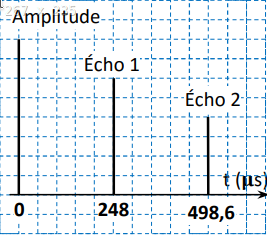
\includegraphics[width=0.27\textwidth]{./img/phys00.png}
  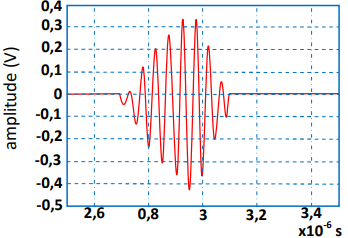
\includegraphics[width=0.27\textwidth]{./img/phys01.png}
  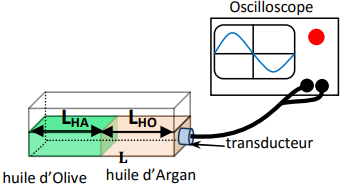
\includegraphics[width=0.27\textwidth]{./img/phys02.png}
\end{center}

\begin{tblr}{c|[dashed]l}
	0.25  & \textbf{1. }Vérifier que la fréquence de l’onde appartient au domaine des ultrasons. \\
  1 & \textbf{2. }Déterminer $V_{HA}$ et $V_{HO}$, les célérités respectives de l’onde dans l’huile d’Argan et l’huile d’Olive. \\
	\end{tblr}
\textbf{3. }Lors d’un contrôle de qualité d’une huile commercialisée en tant
qu’une huile d’Argan, un technicien a pu déterminer la célérité de
l’onde ultrasonore dans cette huile.
Cette célérité vaut $V_{Hc} = 1590 m/s.$  

\begin{wrapfigure}[0]{r}{0.28\textwidth}
  \vspace{0.5cm}
\begin{center}
  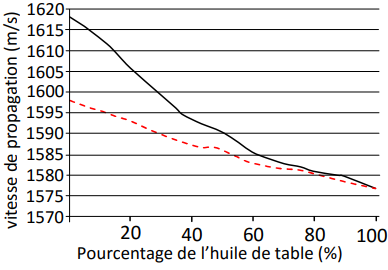
\includegraphics[width=0.28\textwidth]{./img/phys03.png}
\end{center}
\end{wrapfigure}

\begin{tblr}{c|[dashed]l}
1.25  & \textbf{3.1. }Cette huile est-elle une huile d’Argan ou d’Olive ? Justifier\\

1,25 & \textbf{3.2. }Les deux courbes représentent les variations des célérités
des ultrasons dans les deux huiles 

  en fonction du pourcentage
massique de l’huile de table que contient chacune d’elle.

  Laquelle des deux courbes est celle de l’huile d’olive ? Justifier. \\

1,25 & \textbf{3.3. }Calculer le volume de l’huile de table que contient un litre d’huile contrôlée.\\
\end{tblr}

\textbf{Données}:
\begin{itemize}
  \item  Masse volumique de l’huile commercialisée : $\rho_{hc}= 0 ,885 g/mL$
  \item Masse volumique de l’huile de table : $\rho_{hT}=0,895 g/mL$. 
\end{itemize}



\section*{Partie 2 : Détermination de l’indice de réfraction d’un matériau  \dotfill(7pts) }
\emph{Le plexiglas ou le (polyméthacrylate de méthyle) (PMMA) est un matériau aux multiples
applications. Ce thermoplastique, qui peut être moulé, se décline dans de nombreux coloris et sous de
nombreuses formes (panneaux, blocs, tuyaux, barres). Ses qualités de transparence et de résistance
sont exploitées pour fabriquer des hublots d'avions, des vitrages, mais aussi des meubles solides et
design…. }

 Détermination de la longueur d’onde d’une radiation monochromatique
On éclaire une fente de largeur a, par une lumière monochromatique de longueur d’onde dans le vide $\lambda_0$,
et on obtient sur un écran des taches lumineuses séparées par des extinctions (voir fig.1)
Données : L=16,0mm; D=1,50 m ; a=0,100 mm ; c= 3.10 8m/s.

\begin{tblr}{c|[dashed]l}
1  & \textbf{1. } Qu’appelle-t-on ce phénomène ? Quelle est la nature de la lumière mise en évidence ?\\

1,5  & \textbf{2. } Définir une radiation monochromatique. Comment peut-on 

  s’assurer qu’elle est monochromatique ?\\
1,5  & \textbf{3. }  Déterminer la valeur de $\lambda_0$ puis calculer sa fréquence\\
\end{tblr}

\textbf{4. } On intercale un bloc en plexiglas de forme parallélogramme et de largeur D’, tangent au plan de l’écran
(voir fig 2). La largeur de la tache centrale devient L’.
Données : L’ =13 mm ; D’=0,90 m.

\begin{center}
  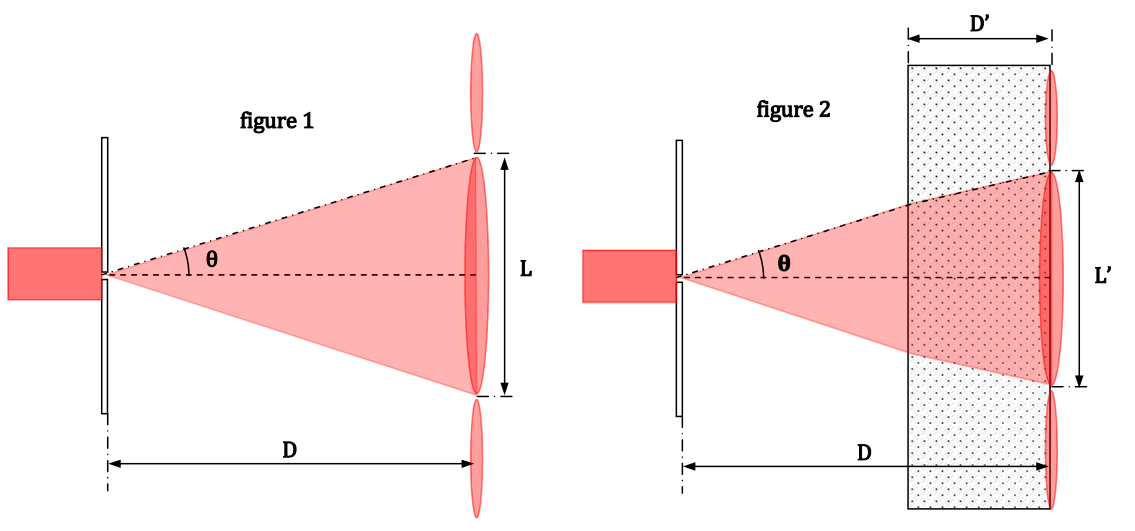
\includegraphics[width=0.7\textwidth]{./img/phys04.png}
\end{center}

\begin{tblr}{c|[dashed]l}
2  & \textbf{4.1. } Appliquer la relation de Descartes de la réfraction puis montrer que l’indice de 

  réfraction du
  plexiglas s’écrit sous forme : $n = \frac{L.D'}{L'.D-L(D-D')}$ \\

2 & \textbf{4.1. } Calculer la valeur de n puis déduire la valeur de la longueur d’onde de la radiation dans

  le plexiglas $\lambda$ . \\

\end{tblr}

\end{document}
